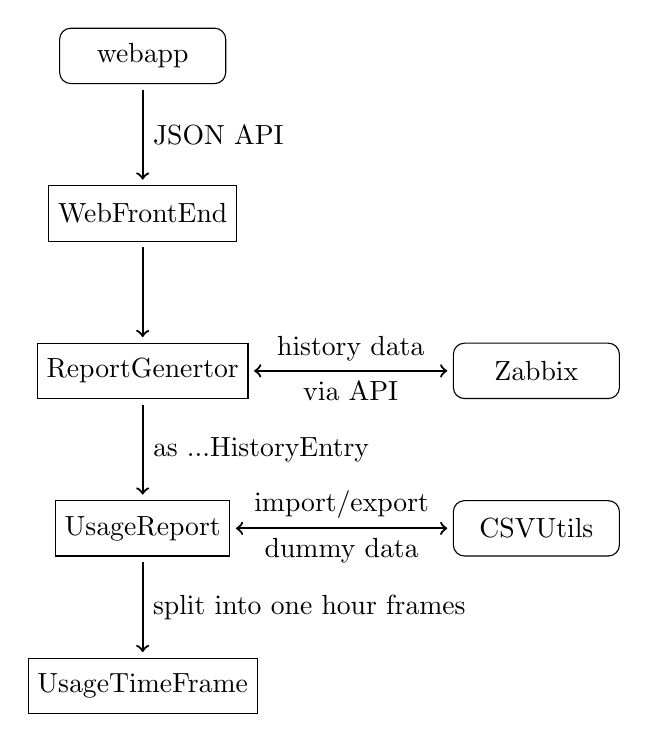
\begin{tikzpicture}
    \tikzset{
        external/.style = {
            rectangle, rounded corners, draw=black,
            minimum width=6em, minimum height=2em, text centered, node distance=5cm
        },
        internal/.style = {
            rectangle, draw=black,
            minimum width=6em, minimum height=2em, text centered, node distance=2cm
        },
        edge/.style = {
            ->, thick, shorten <= 2pt, shorten >= 2pt
        },
        dotted box/.style = {
            rectangle, draw = black, rounded corners, dashed, inner sep=3pt
        }
    };

	\node[internal] (generator) {ReportGenertor};
	\node[internal] (web) [above of = generator] {WebFrontEnd};
	\node[external, node distance = 2cm] (webapp) [above of = web] {webapp};
	\node[external] (zabbix) [right of = generator]  {Zabbix};
	\node[internal] (report) [below of = generator] {UsageReport};
	\node[external] (csv) [right of = report] {CSVUtils};
	\node[internal] (frame) [below of = report]{UsageTimeFrame};

	\draw[edge] (webapp) -- (web) node [midway, right] {JSON API};
	\draw[edge] (web) -- (generator);
	\draw[edge, <->] (generator) -- (zabbix)
		node [midway, above] {history data}
		node [midway, below] {via API};
	
	\draw[edge, <->] (report) -- (csv) 
		node [midway, above] {import/export} 
		node [midway, below] {dummy data};
	
	\draw[edge] (generator) -- (report)
		node [midway, right] {as ...HistoryEntry};
	\draw[edge] (report) -- (frame) 
		node [midway, right] {split into one hour frames};
\end{tikzpicture}